\documentclass{article}%
\usepackage[T1]{fontenc}%
\usepackage[utf8]{inputenc}%
\usepackage{lmodern}%
\usepackage{textcomp}%
\usepackage{lastpage}%
\usepackage[head=40pt,margin=0.5in,bottom=0.6in]{geometry}%
\usepackage{graphicx}%
%
\title{\textbf{Ordenan salida de aire del programa “Gente de Palabra”}}%
\author{Diario El Universal}%
\date{10/10/2018}%
%
\begin{document}%
\normalsize%
\maketitle%
\textbf{URL: }%
http://www.eluniversal.com/el{-}universal/22804/ordenan{-}salida{-}de{-}aire{-}del{-}programa{-}del{-}programa{-}gente{-}de{-}palabra\newline%
%
\textbf{Periodico: }%
EU, %
ID: %
22804, %
Seccion: %
el{-}universal\newline%
%
\textbf{Palabras Claves: }%
NO\_TIENE\newline%
%
\textbf{Derecho: }%
1.7%
, Otros Derechos: %
NO\_TIENE%
, Sub Derechos: %
NO\_TIENE%
\newline%
%
\textbf{EP: }%
SI\newline%
\newline%
%
\textbf{\textit{El conductor del espacio radial, Alonso Moleiro, indicó que la suspensión obedece, según su criterio, a opiniones emitidas sobre la necesidad de “elecciones limpias, decentes y justas”}}%
\newline%
\newline%
%
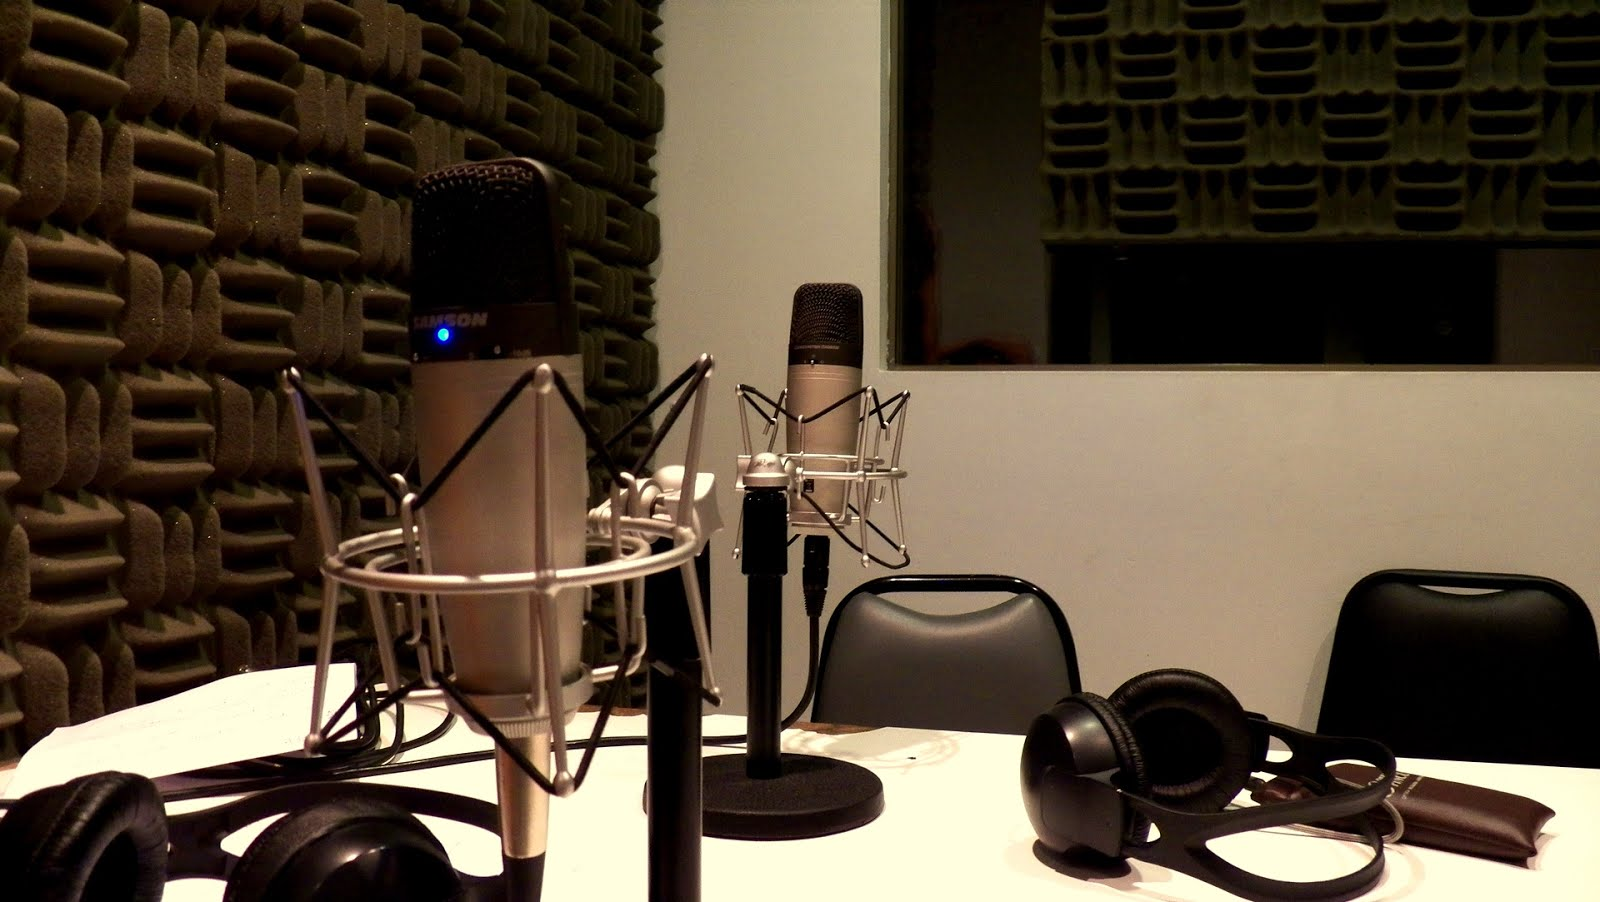
\includegraphics[width=300px]{106.jpg}%
\newline%
%
~Caracas.{-} Este martes se conoció que Conatel ordenó la salida del aire del programa%
\newline%
%
. El espacio transmitido en la 90.3 FM, de la cadena Unión Radio, era conducido por los  comunicadores Alonso Moleiro y Esteninf Olivarez.%
\newline%
%
El periodista informó en su cuenta en la red social Twitter (@amoleiro)  lo siguiente: “Hasta hoy los estuvimos acompañando en \#GenteDePalabra, 90.3 Fm en Caracas, por @Unionradionet. Conatel ha ordenado nuestra salida del aire. Quiero enviar una palabra muy especial de aliento, cariño y reconocimiento a mis compañeros del @Unionradionet, lugar que considero mi casa. A mis productores, Yessica y Luis Ignacio, a Valeria. A mis queridas @MariaFFlores2 y @esteninf y a todos mis compañeros del circuito”.%
\newline%
%
Según indicó Moleiro, “a @Conatel le molestó, entre otras, que yo haya dicho que en este país no se hicieron unas elecciones limpias, decentes y justas, y que la sociedad democrática debería pedir que se repitan, que se hagan, unas verdaderas elecciones presidenciales. Como las de antes”.%
\newline%
%
Agregó que espera continuar “en el país, desde otros espacios, que existen, comprometidos con esta lucha, informando, pero también diciendo lo que pienso, haciendo mi trabajo, mi parte como periodista y como venezolano. Yo no tengo por qué andarme disculpando por expresar mis opiniones. Este país se debe a sí mismo una reflexión muy seria sobre la normalización de la barbarie, la banalización del voto, la confiscación de la soberanía popular, la decencia en la administración y el ejercicio del poder. Los venezolanos deberían poder elegir quién los gobernará”.%
\newline%
%
\end{document}